\chapter{\IfLanguageName{dutch}{Stand van zaken}{State of the art}}%
\label{ch:stand-van-zaken}

\section{Inleiding tot industriele netwerkbeveiliging.}

\subsection{Wat is een firewall}
Volgens \textcite{ciscoFW2025} is de definitie van een firewall `Een netwerkbeveiligingsapparaat dat een vertrouwd intern netwerk scheidt van een extern netwerk dat als onbetrouwbaar wordt beschouwd, zoals bijvoorbeeld het internet.` Het regelt inkomend en uitgaand netwerkverkeer op basis van vooraf ingestelde beveiligingsregels. Firewalls zijn van het grootste belang bij het afschermen van netwerken tegen ongeautoriseerde toegang, schadelijke activiteiten en potentiële bedreigingen.
Op deze manier kan de beheerder van de firewall kunnen beslissen welk verkeer er in en uit zijn netwerk gaat. Hierdoor kan men het interne netwerk beschermen tegen dreigingen van buitenaf.


Volgens \textcite{ciscoFW2025} kan een firewall bestaan in verschillende vormen, binnen deze zelfde bron van Cisco worden er een groot aantal firewalls doorlopen. Een aantal bekende en veelgebruikte firewalls zijn de statefull inspection firewalls, packet filtering firewall's  en NGFW's.
 
Volgens \textcite{goel2014} zullen packet filtering firewalls elk pakket onafhankelijk evalueren, zonder verbindingen bij te houden. Elk pakket zal individueel worden beoordeelt aan de hand van de door de beheerder gedefinieerde regels. Dit vereist vaak aparte regels voor zowel het uitgaand (outbound) als inkomend (inbound) verkeer. De mogelijkheid om te specifieren of een filter inbound of outbound is geeft je grotere controle over waar de router verschijnt in het filterschema , en is zeer handig voor het filteren op routers met meer dan twee interfaces. Als bepaalde pakketten gedropt kunnen worden door een inbound filter op een interface, dan moeten die pakketten niet vermeld te worden in de outbound filters op alle andere interfaces. Men zal dan filters kunnen gaan toepassen voor bepaalde parameters van het pakket zoals source IP adres, destination IP adres en poortnummer maar ook aan de hand van het gebruikte IP protocol. Hoewel deze 'stateless firewalls' vandaag de dag minder vaak gebruikt worden, zijn ze nog steeds aanwezig in sommige netwerkapparatuur, vaak zijn dit switches of routers. Het grootste verschil tussen deze statefull en stateless firewalls is dat de stateless firewalls zoals de naam het zegt geen staten van verbindingen zullen gaan bijhouden, zij zullen regels toepassen op alle pakketten zonder rekening te houden met hun context. \autocite{goel2014}

Volgens \textcite{paloAltoSF2025} zou men dit probleem kunnen oplossen door gebruik te maken van statefull firewalls. In tegenstelling tot stateless inspectie die elk pakket afzonderlijk behandelt, ziet de statefull firewall het netwerkverkeer als een continue stroom. Dit doet hij onder andere door te kijken naar de 'three way handshake'. Dit maakt het mogelijk om patronen te detecteren die wijzen op potentiële bedreigingen. Stateful inspection analyseert de header van het pakket om te bepalen of het deel uitmaakt van een bestaande conversatie. Als een pakket niet overeenkomt met een bestaande verbinding, dan wordt het geëvalueerd aan de hand van de vooraf beschreven firewallregels om te beslissen of het doorgelaten moet worden. Volgens Palo Alto zouden statefull firewalls actieve verbindingen intelligenter beheren, waardoor de netwerkbronnen efficiënter gebruikt kunnen worden. Pakketten van vertrouwde verbindingen hoeven op deze manier niet voortdurend opnieuw geëvalueerd te worden. Dit zorgt ervoor dat de verwerkingslast wordt verlaagt en de doorvoersnelheid wordt gemaximaliseerd. 

Vandaag de dag wordt er als maar meer gebruik gemaakt van Next Generation Firewalls (NGFW’s) die diepe packet inspection uitvoeren en op basis hiervan zullen beslissen of een packet wordt geblokkeerd of niet. Sedert 2020 maken deze NGFW’s ook gebruik van Artificiële Intelligentie (AI). \autocite{Ahmadi2023}. Firewalls die gebruik maken van AI genereren beveiligingsmaatregelen en dwingen deze af op basis van het continue netwerkverkeer waardoor de blootstelling aan nieuwe bedreigingen aanzienlijk wordt verminderd. \autocite{PaloAltoFW2024}

Ondanks de snelle evolutie van firewalls blijft een groot struikelblok bij het toepassen hiervan de complexiteit van bedrijfsnetwerken. Volgens \textcite{Bringhenti2023} wordt het configureren van security functies typisch nog steeds manueel gedaan. Maar omdat moderne netwerken zodanig complex en dynamisch zijn, is de manuele configuratie hiervan niet haalbaar. Dit zorgt ervoor dat het kiezen van een gepaste firewall niet alleen draait om de manier waarop mogelijke threats worden afgehandeld, maar ook de manier waarop de automatisatie en configuratie zullen kunnen worden toegepast.



\subsection{Evolutie van firewalls}
Firewalls bestaan al sinds de jaren’ 80, toendertijd deden firewalls slechts enkel aan basic packet filtering. Sindsdien zijn firewalls steeds blijven evolueren, enerzijds door de groeiende digitalisering en anderzijds door de grotere cyberdreigingen tegen industriële infrastructuur van productiebedrijven \autocite{Wusteney2021}. 
Vandaag de dag wordt er gebruik gemaakt van Next Generation Firewalls (NGFW’s) die diepe packet inspection uitvoeren en op basis hiervan beslissen of een pakket wordt geblokkeerd of niet. Sedert 2020 maken deze NGFW’s ook gebruik van Kunstmatige Intelligentie (AI) \textcite{Ahmadi2023}. Firewalls die gebruik maken van AI genereren beveiligingsmaatregelen en dwingen deze af op basis van het continue netwerkverkeer, waardoor de blootstelling aan nieuwe bedreigingen aanzienlijk wordt verminderd \textcite{PaloAltoFW2024}.

  
\subsection{Belang van cybersecurity in een productieomgeving}

De golfkartonindustrie is sterk afhankelijk van onderling verbonden systemen, waardoor cybersecurity essentieel is. OT zal belangrijke productieprocessen gaan beheren die grondstoffen omzetten in nauwkeurige verpakkingen van hoge kwaliteit, zoals het snijden en printen van golfkarton en zorgt zo voor efficiëntie en kwaliteit. Ook zal real-time bewaking binnen deze systemen de productkwaliteit op peil houden en zo verspilling minimaliseren. Door het monitoren van de machines zal er efficiënter kunnen worden ingespeeld op het onderhoud waardoor deze machines een langere levensduur zullen hebben. Naarmate OT-systemen en Cyber Physical Systems (CPS) meer met elkaar verbonden raken, is het van cruciaal belang om ze te beveiligen tegen cyberbedreigingen. Een inbreuk kan de productie verstoren, de kwaliteit in gevaar brengen en gevoelige informatie blootleggen. In de huidige industrie beschermt robuuste OT beveiliging zowel de productie-integriteit als de bedrijfscontinuïteit. \autocite{fefco2025}

Deze toename in connectiviteit tussen systemen zorgt er niet alleen voor dat nieuwe eisen nodig zijn op het vlak van cybersecurity, maar heeft ook een impact op de bescherming van het ICS zeker als we weten dat de beveiliging van het ICS lange tijd als minder belangrijk werd beschouwd. Vaak werd er gewerkt met "security through obscurity" wat betekent dat systemen werden beschermd door informatie geheim te houden in plaats van echte beveiligingsmaatregelen te implementeren. Dit werkte redelijk goed voor oudere systemen, omdat ze enkel in contact stonden met apparaten vanop het eigen netwerk en amper verbonden waren met apparaten buiten hun netwerk. Bij de derde en tevens ook nieuwste generatie ICS is deze aanpak echter veel minder effectief. Moderne systemen maken gebruik van open technologieën om te communiceren met andere niet-ICS netwerken, waaronder het internet. Hierdoor is de beveiliging door onduidelijkheid niet langer voldoende, omdat aanvallers steeds beter bekend zijn met de gebruikte technologieën en kwetsbaarheden makkelijker kunnen vinden. \autocite{knowles2015}

Ondanks de snelle evolutie van firewalls blijft een groot struikelblok bij het toepassen hiervan de complexiteit van bedrijfsnetwerken. Volgens Bringhenti e.a. (2023) wordt het configureren van security functies typisch nog steeds manueel gedaan. Maar omdat moderne netwerken zodanig complex en dynamisch zijn, is de manuele configuratie hiervan niet haalbaar. Het kiezen van een gepaste firewall draait niet alleen om hoe mogelijke bedreigingen worden afgehandeld, maar ook om hoe automatisatie en configuratie kunnen worden toegepast.


\subsection{Verschil tussen IT en OT infrastructuur en beveiliging}

OT omvat een breed scala aan programmeerbare systemen en apparaten die direct of indirect in interactie zullen gaan met de fysieke omgeving. Veelvoorkomende OT-toepassingen zijn Supervisory Control and Data Acquisition (SCADA) voor grootschalige procesmonitoring, Programmable Logic Controllers (PLC) voor de besturing van machines en productielijnen. Daarnaast omvat OT ook de Industrial Internet of Things (IIoT) voor het verbinden van industriële apparaten en sensoren. OT kan worden ingezet voor het monitoren, besturen en automatiseren van industriële processen, transport en energiebeheer. Deze systemen bestaan uit verschillende onderdelen met elk eigen functies. Zoals mechanische, elektrische, hydraulische en pneumatische onderdelen, die samenwerken om bepaalde doelstelling te behalen. \autocite{Stouffer2023}.

Hoewel OT-systemen traditioneel geïsoleerd waren, worden ze steeds vaker gekoppeld aan IT-netwerken, wat voordelen biedt op het gebied van efficiëntie en gegevensanalyse, maar ook nieuwe beveiligingsrisico’s met zich meebrengt. Daarom is een robuuste beveiligingsarchitectuur essentieel voor het waarborgen van de betrouwbaarheid en integriteit van OT-systemen. \autocite{Stouffer2023}.

\section{Firewall technologieen en hun rol in de ICS beveiliging}

\subsection{Sophos en Palo Alto firewalls binnen het VPK netwerk.}
Om het onderzoek in deze bachelorproef goed te begrijpen, is een basiskennis van tweefirewall merken essentieel: Sophos en Palo Alto. Sophos firewalls staan erom bekend dat ze zeer gebruiksvriedelijke userinterfaces en geintegreerde beveiligingsoplossingen hebben. Ze bieden een breed scala aan functies aan waaronder deep packet inspection (DPI), intrusion prevention system (IPS), geavanceerde dreigingsanalyse en synchronisatie met andere Sophos producten via Synchronized Security. \autocite{Phipps2024}

Palo Alto firewalltoepassingen onderscheiden zich dan weer door hun geavanceerde applicatie- en identiteitsgebaseerde beveiligingsfuncties. Daarnaast biedt Palo Alto ook krachtige IPS en IDS toepassingen die het bedrijf kunnen beschermen tegen malware en andere cyberdreigingen. Palo Alto geeft ook de mogelijkheid om gebruik te maken van hun cloud based beheerplatform met de naam Strata Cloud. Deze beveiligingssuite zorgt ervoor dat bedrijven hun infrastructuur kunnen beschermen ongeacht of ze zich on-premises, in de cloud of in hybride omgevingen bevinden. \autocite{shread2023}

Er zijn wel degelijk een aantal grote verschillen tussen deze twee firewall vendors. Sophos firewalls zijn bijzonder gebruiksvriendelijk, met een eenvoudig beheerplatform via Sophos Central, wat ideaal is voor kleinere bedrijven. Palo Alto biedt meer geavanceerde functionaliteiten, maar vereist een diepere technische kennis voor configuratie en beheer van de firewall. Beide firewalls hebben een cloud based beheerplatform. Echter zal Sophos Central zich meer richten op eenvoudig beheer, terwijl Palo Alto Strata een uitgebreider platform is voor hybride en multi-cloud omgevingen. \autocite{paloGuard2025} 

Echter wil dit niet direct zeggen dat de ene firewall voor alle use-cases beter is dan de anderefirewall. Het kiezen van het juiste merk van firewall hangt heel erg af van de schaal van hetnetwerk waarin deze zich zal bevinden. Ook de ervaring van het netwerkteam dat de infrastructuur beheerd kan een grote rol spelen in de keuze. Heeft het team al eerder gewerkt met firewalls van een bepaalde vendor? Bestaat het team uit ervaren medewerkers of eerder uit junior profielen? Dit zijn allemaal zaken die je in je achterhoofd moet houden bij het kiezen van een firewall toepassing.



\subsection{Segmentatie als beveiligingstoepassing}
Firewalls worden gebruikt door organisaties om interne infrastructuur te beschermen tegen ongeautoriseerde toegang door data te inspecteren en bepaalde beveiligingsmaatregels toe te passen. Echter zal een firewall ook kunnen worden gebruikt voor het verdelen van het netwerk in meerdere delen die elk verschillende beveiligingseisen hebben. Een multinational zoals VPK heeft honderden firewalls waardoor de configuratie en locatie van de firewall’s in het netwerk cruciaal zijn. Om deze honderden firewalls correct te segmenteren heeft men een plan nodig die op iedere firewall zal worden uitgevoerd. Op deze manier zal iedere firewall op dezelfde manier geconfigureerd zijn. En wordt de kans op afwijkingen van de gewenste werking beperkt. Ook zal het beheren van de firewalls na de installatie een stuk vlotter gaan als alle firewalls in een uniforme manier zijn opgezet.
Twee veelgebruikte strategieën bij het beveiligen van een netwerk zijn gelaagde beveiliging en segmentatie. Gelaagde beveiliging, ook wel gekend als Defence in Depth (DD), zorgt ervoor dat een netwerk meerdere beveiligingslagen bevat. Iedere laag heeft apparte beveiligingsmaatregelen. Dit zorgt ervoor dat als een attacker door één van de lagen penetreert, de andere lagen nog steeds het netwerk zullen beveiligen. \autocite{FortinetDE2025} Bij netwerksegmentatie wordt de infrastructuur ingedeeld in verschillende zones, elke zone is beschermd door één of meerdere firewalls die afgstemd zijn op specifieke beveiligingseisen van die welbepaalde zone. Echter zijn er geen duidelijke richtlijnen aanwezig om segmentatie op een efficiënte manier aan te pakken. Hierdoor kan dit soms uitdagend zijn. \autocite{Mhaskar2021}
Een andere manier van segmentatie is het gebruiken van een DMZ (Demilitarized Zone). Dit is een soort van subnetwerk dat zich tussen het interne LAN en het WAN bevindt. In dit netwerk zullen publiekgerichte services beschikbaar zijn. Enkele voorbeelden van services die vaak in de DMZ gehost zijn, zijn de DNS server, mailserver en webserver. \autocite{Patel2020}



\section{ICS architectuur binnen een industriële omgeving}

\subsection{Doel van SWOT en RASCI binnen een vergelijkende studie}
SWOT staat voor strenghts, weakneses, opportunities and threats en is een tool die wordt gebruikt om belangrijke interne en externe factoren te begrijpen die een organisatie of project beïnvloeden. SWOT werd ontwikkeld door Albert Humphrey in de jaren '60 en '70. Een SWOT analyse helpt bij het maken van strategische keuzes door het identificeren van sterke en zwakke punten, maar ook door externe kansen en bedreigingen. Hoewel het maken van een SWOT analyse eenvoudig lijkt, vereist een goede SWOT analyse tijd, veel tijd en middelen. dit komt omdat het vinden van de juiste factoren niet altijd eenvoudig of straight forward is. Onjuiste aannames kunnen leiden tot vertragingen in strategische keuzes.\autocite{cipd2025}

SWOT analyses hebben verschillende voor en nadelen. De grootste voordelen die een SWOT analyse biedt is de graad waarin het in een bedrijf kan worden toegepast. Het kan gebruikt worden voor het beoordelen van een kleinschalig project, maar evengoed voor het beoordelen van de volledige bedrijfsstrategie. Ook is het makkelijk om op te stellen. Je hebt geen uitgebreide wiskundige kennis nodig voor het opstellen van het diagram. Echter zijn er ook een aantal nadelen aan verbonden. Zo kan het zijn dat een SWOT analyse wordt opgesteld op basis van assumpties en vooroordelen en niet op basis van feiten. Een analyse die op deze manier wordt gedaan, is in de praktijk echter niet zo waardevol. \autocite{sarsby2012}


Volgens \textcite{putman2024} is het RASCI-model een tool die wordt gebruikt om rollen en verantwoordelijkheden binnen een project of organisatie te verduidelijken. Het staat voor responsible, accountable, supporting, consulted en informed. Het model helpt bij het structureren van verschillende taken en bevoegdheden. Het model wordt vaak gebruikt binnen het projectmanagement om onduidelijkheden omtrent bevoegdheden te voorkomen. Binnen een grootschalige industriële omgeving zoals die van VPK kan RASCI bijdragen aan een vlotte en efficiënte samenwerking tussen IT en OT teams door duidelijk vast te leggen wie verantwoordelijk is voor implementatie, wie eindverantwoordelijk is, wie ondersteuning biedt, wie geraadpleegd moet worden en wie op de hoogte gehouden moet worden. Vaak wordt er echter gebruik gemaakt van het RACI model, hierbij zal de supporting role van het RASCI model worden weggelaten. Deze methode wordt vooral gebruikt binnen organisaties met een minder complexe samenwerkingsstructuur. \autocite{harkhoe2025}


\subsection{Het PROFIBUS protocol}
PROFIBUS, een afkorting voor Process Field Bus, is een gestandaardiseerd communicatieprotocol dat in 1989 werd geïntroduceerd. Het kan gebruikt worden als een digitale netwerkoplossing voor het automatiseren van verschillende processen binnen productiesites. \autocite{Profibus2022}
Ook binnen VPK wordt er nog steeds gebruik gemaakt van dit protocol.
Het protocol zorgt ervoor dat er een gestandaardiseerde applicatie-onafhankelijke communicatie mogelijk is tussen een groot aantal apparaten van verschillende fabrikanten. \autocite{Profibus2022}
PROFIBUS is ontworpen om real-time communicatie in industriële netwerken te ondersteunen. Het protocol geeft prioriteit aan de beschikbaarheid van de apparaten, wat destijds in 1980 de belangrijkste “beveiligingsdoelstelling” was. Echter, met de toenemende blootstelling van industriële netwerken aan andere openbare netwerken, zijn er beveiligingsrisico’s aan het licht gekomen binnen het PROFIBUS protocol. Onderzoek heeft aangetoond dat er kwetsbaarheden bestaan die kunnen worden misbruikt als er geen gepaste beveiligingsmaatregelen worden genomen. \autocite{Watson2017}
Het is belangrijk op te merken dat hoewel PROFIBUS nog steeds veel wordt gebruikt, er een verschuiving plaatsvindt naar op Ethernet gebaseerde protocollen zoals PROFINET. Deze protocollen bieden hogere snelheden en verbeterde integratie met moderne industriële netwerken. Toch blijft PROFIBUS een robuuste en betrouwbare oplossing voor vele automatiseringstoepassingen. \autocite{Aminaie2020}


\subsection{Overzicht van de verschillende ICS componenten}
Binnen eender welke productiesite van VPK wordt er gebruikgemaakt van veel verschillende componenten die deel uitmaken van de OT omgeving. Daarom is het belangrijk om te weten uit welke componenten de algemene VPK productie-site is opgebouwd. 

Omdat de meeste productiesites vandaag de dag nog niet 100 \% autonoom kunnen werken zonder tussenkomt van een operator die de machine bestuurd zal er steeds nood zijn aan een bepaalde manier om input van de operator door te geven aan de machine. Dit zal vaak gebeuren op basis van een HMI (Human-Machine Interface). 
Volgens \textcite{Nist2025} is een HMI De hardware of software waarmee een operator communiceert met een controller. Een HMI kan variëren van een fysiek bedieningspaneel met knoppen en indicatielampjes tot een industriële pc met een grafisch kleurenscherm waarop speciale HMI-software draait. De operatoren kan via deze interface bepaalde bedieningen uitvoeren op de machine. In andere woorden zal een HMI er voor zorgen dat bepaalde configuraties die de operator wil maken op een efficiënte en duidelijke manier voor de operator worden doorgevoerd naar de machine. 
Nu zal de HMI niet enkel worden gebruikt voor het invoeren van data voor een operator, hij kan ook worden gebruikt voor het tonen van belangerijke informatie van de machine aan de operator zoals grafieken, diagrammen en digitale dashboards. \autocite{Inductive2025}
Volgens \textcite{Copadata2025} zou je technisch gezien de term HMI kunnen toepassen op elk scherm dat iemand gebruikt voor interactie met een apparaat, maar de term wordt meestal gebruikt om schermen te beschrijven die in industriële omgevingen worden gebruikt.

\begin{figure}[H]
    \centering
    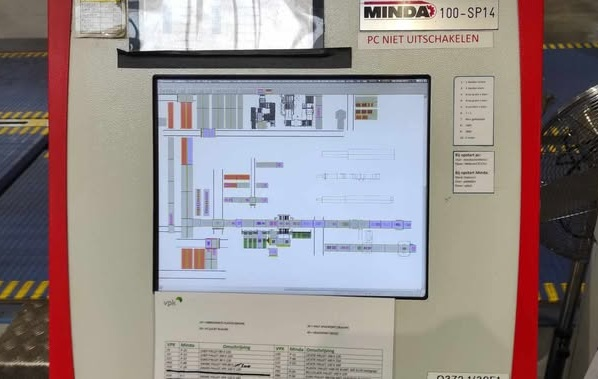
\includegraphics[width=0.8\textwidth]{fotos/Minda_HMI.jpg}
    \caption[Minda HMI]{\label{fig:grail}Een Minda HMI voor het besturen van het geautomatiseerd Minda magazijn.}
\end{figure} 

Een PLC is een apparaat dat cruciaal is binnen eender welke productiesite. De PLC is in staat om op basis van bepaalde invoerapparaten zoals sensoren beslissingen te maken aan de hand van “ladder logical”. Deze beslissingen triggeren dan weer acties die zullen worden ondernomen door aangesloten output apparaten zoals relais, LED’s, pneumatica en aandrijvingen \autocite{unitronics2025}.
Vaak zal de besturing van de PLC gebeuren aan de hand van een HMI, echter zal de operator van de HMI geen daadwerkelijke code moeten schrijven, maar kan hij bepaalde data zien of handelingen uitvoeren via speciale software die beschikbaar is op de grafische gebruikersinterface van de HMI. 
Echter is het verzamelen van data aan de hand van PLC’s en andere slimme industriele sensoren niet genoeg, men moet deze data kunnen omvormen naar nuttige informatie die gebruikt kan worden om het gebruiksgemak en de efficiëntie te verhogen. 

\begin{figure}[H]
    \centering
    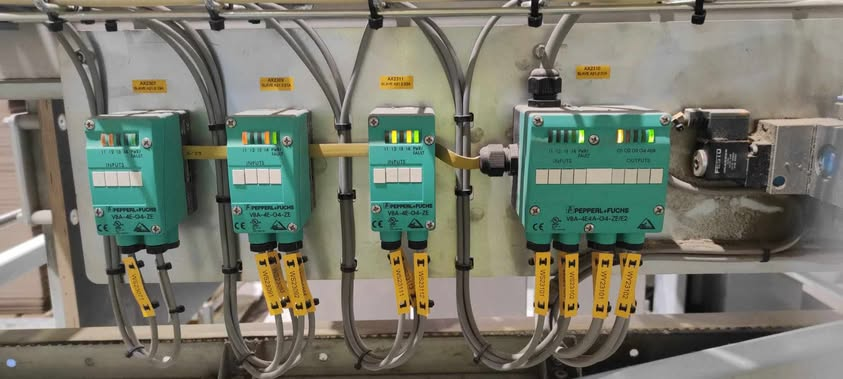
\includegraphics[width=0.8\textwidth]{fotos/PLC_pneumatica.jpg}
    \caption[Pneumatica PLC]{\label{fig:grail}De pneumatische onderdelen van een PLC sturing binnen een VPK productiesite}
\end{figure} 

Een manier om de efficiëntie te verhogen is door gebruik te maken van SCADA-systemen. 
Deze systemen zullen gebruik maken van HMI’s om de verkregen data van de verschillende sensoren omvormen, om op hoog niveau controle, beheer en toezicht te houden op industriële processen. SCADA netwerken zijn cruciaal voor industriële activiteiten, maar bestaan uit verouderde hardware en software die gemakkelijk gehackt kunnen worden, waardoor SCADA-beveiliging steeds belangrijker wordt.\autocite{FortinetSC2025}. SCADA moet dus eigenlijk niet gezien worden als een onderdeel van het ICS maar eerder als een type van ICS. 
Volgens \textcite{Mhaskar2021} is ICS een verzamelnaam voor verschillende soorten apparaten, systemen, netwerken en besturingen die worden gebruikt om industriële processen te bedienen en/of te automatiseren. Wat SCADA in deze context zal doen is het beheren en samenbrengen van allerlei databronnen om deze te verwerken.


\subsection{Zones, conduits en Purdue model voor ICS netwerken.}
Security zones zijn groepen systemen en componenten die functioneel, logisch of fysiek bij elkaar horen en dezelfde beveiligingseisen delen. Denk bijvoorbeeld aan een zone met alle PLC’s binnen de productie van een site of een zone met alle HMI’s en camerafeeds in een controlekamer. Door systemen op deze manier te groeperen, wordt het eenvoudiger om gerichte beveiligingsmaatregelen toe te passen en risico’s beheersbaar te houden. De communicatie tussen deze zones verloopt via conduits, dit zijn de verbindingslijnen tussen verschillende zones. Dit kunnen fysieke of logische verbindingen zijn, zoals ethernetnetwerken,fiber kabels of VPN-tunnels . Conduits bepalen welke informatie tussen zones mag worden uitgewisseld en zorgen ervoor dat alleen geautoriseerde communicatie tussen twee apparaten zal plaatsvinden. Op deze manier wordt de ongewenste toegang tot verschillende systemen zo minimaal mogelijk gehouden. Zodat de potentiele aanval niet zomaar van de ene naar de andere zone kan overslaan. \autocite{Dragos2023}
Je mag het ontwerpen van zones en conduits niet zien als een gesloten process. Na verloop van tijd veranderen er zaken in de architectuur waardoor de zones en conduits mogelijk niet meer optimaal zijn verdeeld. Daarom is het belangrijk om continue dit process the reevalueren en tijdig aanpassingen uit te voeren. Het is de bedoeling dat je voortdurend verbeteringen aanbrengt, waarbij de risicos op aanvallen worden verlaagd. \autocite{Incibe2018}
Een vaak gebruikt model waarbij we het netwerk zullen opdelen in verschillende zones is het Purdue model. Dit is een model dat ontwikkeld is aan de Purdue Universiteit in de Verenigde Staten begin jaren `90. Volgens \textcite{Mathezer2021}heeft het model als doel om best practices te definiëren voor de relatie tussen industriële besturingssystemen en bedrijfsnetwerken of met andere woorden tussen IT en OT. 

Volgens \textcite{Commers2025} zou het purdue model systemen onderverdelen in vijf verschillende niveaus, de niveaus 0 tot en met 2 hebben betrekking op real-time besturing en automatiseringsprocessen, waaronder sensoren, actuatoren en besturingssystemen zoals PLC’s . Niveau 3 richt zich op Manufacturing Operations Systems (MOS), die toezicht houden op de productie-uitvoering, gegevensverzameling en kwaliteitscontrole. Niveau 4 houdt zich bezig met bedrijfssystemen zoals ERP toepassingen. Waar productieschema's, voorraden en andere processen op hoog niveau worden beheerd.

Dit hiërarchische model bevordert duidelijkheid en scheiding van functies, waardoor betere communicatie tussen IT en OT mogelijk wordt. Het wordt veel gebruikt in industriële omgevingen om een soepele werking te garanderen, de cyberveiligheid te verbeteren en initiatieven voor digitale transformatie te begeleiden, waaronder de toepassing van Industrie 4.0-technologieën, zoals het IIoT. \autocite{Commers2025}

Ondanks de vele dynamische cyberdreigingen in het huidige OT-landschap blijft het Purdue-model een hoeksteen voor het beveiligen van het OT-netwerk. Het grote voordeel van dit model is dat de schaalbaarheid het geschikt maakt voor bedrijven met een grotere omvang. Ondanks de wat oudere leeftijd van dit model en de steeds geavanceerdere aanvallen op OT-netwerken, blijven de kernprincipes zoals segmentatie, in-depth defence en risicobeheer essentieel voor het beperken van cyberrisico’s in industriële omgevingen. In-depth defence zorgt ervoor dat meerdere beschermingslagen, zoals firewalls, toegangscontrole en monitoring, samenwerken om aanvallen te blokkeren. Je zal als het ware meerdere lagen aan beveiliging implementeren. Risicobeheer richt zich op het identificeren en beperken van bedreigingen om de impact op kritieke systemen binnen VPK te minimaliseren.

\subsection{Oplossingen voor de complexiteit van een firewall implementatie.}

Volgens \textcite{Bringhenti2023} wordt het configureren van security functies typisch nog steeds manueel gedaan. Maar omdat moderne netwerken zodanig complex en dynamisch zijn, is de manuele configuratie hiervan niet haalbaar. Het kiezen van een gepaste firewall draait niet alleen om hoe mogelijke bedreigingen worden afhandelen, maar ook om hoe automatisatie en configuratie kunnen worden toegepast.

Er is een manier om de complexiteit van een groot bedrijfsnetwerk te verminderen door het toepassen van netwerksegmentatie \autocite{Bringhenti2023}. Hierdoor wordt het schrijven van veiligheidsmaatregelen beheersbaar en kunnen er robuuste security policies worden opgesteld voor het netwerk. Palo Alto Networks is een van de marktleiders op het vlak van cybersecurity-toepassingen, waaronder NGFW’s, cloud-based security services, advanced endpoint protection en threat intelligence \autocite{TechnicalWhitepaper2014}.

Palo Alto heeft bijvoorbeeld een cloud-based malware protection engine genaamd WildFire. WildFire is een Intrusion Detection System (IDS) die bestanden, die als mogelijke dreiging worden gecategoriseerd, uitvoert in een sandbox omgeving. Hier worden de dreigingen geanalyseerd met behulp van machine learning algoritmes die gedrag en patronen detecteren die indicatief zijn voor kwaadaardige activiteit \autocite{PaloAltoWF2024}.




\section{verschillende dreigingen op het ICS}

\subsection{Specifieke ICS aanvallen}

De laatste jaren is het cyberbeveiligingsbewustzijn sterk gegroeid, dit komt onder andere door verschillende grootschalige cyberaanvallen die de afgelopen jaren plaatsvonden. Een van de eerste grootschalige aanvallen die het gedachtegoed rond cybersecurity heeft veranderd is het Stuxnet-incident in 2010, dat gericht was op de Iraanse kerncentrale Natanz en ongeveer 25\% van de centrifuges voor uraniumverrijking beschadigde. \autocite{Zetter2014}. 

Ook viel de Shamoon-malware in 2012 het Saudische oliebedrijf Saudi Aramco en het Qatarese aardgasbedrijf RasGas aan, waarbij data werd vernietigd en geïnfecteerde systemen onbruikbaar werden \autocite{Hemsley2018}.
In diezelfde bron wordt er ook gesproken over een van de eerste publieke bekende cyberaanvallen op het elektriciteitsnet, een aanval op een Oekraïense energiebedrijf in 2015 ervoor zorgde dat bijna een kwart miljoen mensen zonder elektriciteit kwamen te zitten.

Echter zijn niet alle cyberaanvallen succesvol, volgens \textcite{Margolin2021} zou februari 2021 de Bruce T. Haddock Water Treatment Plant in Florida gehackt zijn door cybercriminelen. Die plant gebruikte een verouderd besturingssysteem waardoor de hacker toegang kreeg tot het computersysteem en de chemische niveaus van de watervoorziening kon wijzigen. De aanval werd ontdekt nog voordat er grote schade kon worden aangebracht.



Volgens \textcite{Morgan2024} werd de schade die cyberattacks aangericht zouden hebben in 2024 geschat op 9,5 biljoen dollar. Nu is de schatting voor de schade die ze zullen aanrichten in 2025 geschat op 10,5 biljoen dollar, dat is een steiging van maar liefst 15\% . Dit maakt dat cybercriminaliteit de op twee na grootste economie ter wereld is, na de VS en China.

\subsection{Insider threats}
Bij het opstellen van een cybersecurity plan wordt er vaak rekening gehouden met twee verschillende soorten threats. Aan de ene kant heb je de insider threats. Dit zijn dreigingen die worden veroorzaak door insiders. Volgens \textcite{Cisa2025} is een insider een persoon die geautoriseerde toegang heeft of had tot kennis van de middelen van een organisatie, zoals personeelsbestanden, faciliteiten, informatie, apparatuur, netwerken en systemen. In diezelfde bron worden een aantal voorbeelden gegeven van insider threats: Een persoon die de organisatie vertrouwt, inclusief werknemers, leden van de organisatie en personen aan wie de organisatie gevoelige informatie en toegang heeft gegeven. In dit geval gaat het over een werknemer die legitieme toegang heeft tot gevoelige informatie over het bedrijf.

Alhoewel dat de insider threats niet zo vaak aan bod komen in het nieuws brengen ze gemiddeld wel het meeste schade toe aan de organisatie. Volgens \textcite{ibm2024} leidden aanvallen van kwaadwillende insiders tot de hoogste kosten, gemiddeld 4,99 miljoen dollar. Andere dure aanvalsvectoren waren de compromisen van zakelijke e-mail, phishing, sociale engineering en gestolen of gecompromitteerde credentials. 

Volgens \textcite{Cisa2025} kan je de verschillende vormen van insider threats opdelen in drie categorieën. De eerste categorie `onopzettelijke dreigingen` komt vooral tot stand door de nalatigheid van de gebruikers.  Hoewel deze personen bekend zijn met de beveiligingsregels, negeren ze deze bewust. Voorbeelden zijn het toestaan van ongeautoriseerde toegang, het kwijtraken van gevoelige gegevens of het niet installeren van beveiligingsupdates. Echter is dit niet de enige vorm van onopzettelijke dreigingen. De gebruiker kan ook per ongeluk bepaalde acties uitvoeren waardoor de cybersecurity van het bedrijf in gevaar gebracht wordt. Dit gaat dan vaak over fouten zoals het per ongeluk verzenden van vertrouwelijke informatie naar een verkeerde ontvanger door bijvoorbeeld een schrijffout in een e-mail adres, het openen van phishingmails of het onjuist verwerken van gevoelige documenten.

Aan de andere kant heb je ook de opzettelijke bedreigingen, vaak zijn dat acties die worden ondernomen om een organisatie schade toe te brengen voor persoonlijk voordeel of om te handelen op basis van een persoonlijke grief. Veel insiders zijn bijvoorbeeld gemotiveerd om “wraak te nemen” vanwege een waargenomen gebrek aan erkenning of door ontslag. Hun acties kunnen bestaan uit het lekken van gevoelige informatie, het lastigvallen van medewerkers, het saboteren van apparatuur, het plegen van geweld of het stelen van bedrijfseigen gegevens of intellectueel eigendom in de vermeende hoop hun carrière te bevorderen.\autocite{Cisa2025}

De derde categorie kan gezien worden als een collectie van alle andere minder voorkomende threats. Een van deze threats zijn bedreigingen van derden dit zijn meestal aannemers of verkopers die formeel geen deel zijn van een organisatie, maar die op een bepaalde manier toegang hebben gekregen tot faciliteiten, systemen of netwerken. \autocite{Cisa2025}



\subsection{Verschillende soorten cyberattacks}
Het gebruiken van online tools en het uitbuiten van kwetsbaarheden in verschillende computersystemen om zo geld te verdienen is geen nieuw begrip. Het zit zelfs zo dat nog voor men computersystemen had zoals we deze vandaag kennen er al verschillende elektronische communicatie systemen werden gebruikt voor het stelen van informatie. Volgens \textcite{Monroe2025} zou de eerste cyberaanval hebben plaatsgevonden in 1834, in deze cyberaanval zouden twee dieven financiële data hebben gestolen door het Franse telegraaf systeem te hacken. 

Sindsdien is het scala aan verschillende types van cyberdreigingen steeds uitgebreid. Een van de meest gebruikte en makkelijkste manieren om toegang te verkrijgen tot bepaalde systemen is phising, volgens \textcite{jagatic2007} is phishing een vorm van misleiding waarbij een aanvaller op frauduleuze wijze gevoelige informatie van een slachtoffer probeert te verkrijgen door zich voor te doen als een betrouwbare entiteit. Een phisher die zich bijvoorbeeld voordoet als een groot bankbedrijf zal een redelijke kan opopbrengst hebben, ondanks dat hij weinig tot niets weet over de ontvanger. 

In het algemeen gebeurt een phising aanval in vier verschillende stappen. Eerst zal de aanvaller het vertrouwen van het slachtoffer proberen te winnen door zich voor te doen als een betrouwbare persoon of organisatie door gebruik te maken van valse websites, e-mails of applicaties, zodat het slachtoffer gewenste acties uitvoert, zoals het klikken op links of beantwoorden van een e-mail. Vervolgens zal er een doorverwijzing plaatsvinden, waarbij het slachtoffer via een link op een phishingwebsite terechtkomt die vaak exact hetzelfde eruitziet als de legitieme website en daar zijn inloggegevens invoert. In de derde stap verkrijgt de aanvaller deze gegevens via een formulier/website of direct via mail. Tot slot voert de aanvaller identiteitsfraude of financiële fraude uit met de verkregen informatie. \autocite{varshney2024}

Echter zal niet elke cyberaanval gefocust zijn op het verkrijgen van informatie die verder verwerkt kan worden. Er zijn ook verschillende cyberaanvallen waarbij de focus wordt gelegd op het verstoren van de service die bepaalde systemen bieden. Een van de meest bekende aanvallen van dit type is de DDoS (Distributed Denial of Service) attacks. Volgens \textcite{Baker2024} is een DDoS aanval een kwaadaardige, gerichte aanval die een netwerk overspoelt met valse verzoeken om de bedrijfsactiviteiten te verstoren. Hierdoor zal de server die deze verzoeken zal verwerken overbelast geraken en geen andere legitieme verzoeken meer kunnen verwerken. Hierdoor kunnen gebruikers geen algemene taken uitvoeren, zoals toegang krijgen tot hun e-mail inbox, websites of andere bronnen die worden beheerd door een aangetaste computer of een aangetast netwerk. Omdat er op deze manier geen gegevens worden verkregen kan het meestal worden opgelost zonder losgeld te betalen. Echter kost het de organisatie tijd, geld en andere middelen om kritieke bedrijfsactiviteiten te herstellen.

Omdat cyberaanvallen op industriële netwerken vaak worden gepleegd door ervaren hackers is het belangrijk om de verschillende aansvalsmethoden die gebruikt kunnen worden en de verschillende stadia die doorlopen worden te begrijpen. We kunnen verschillende cyberaanvallen vaak gaan onderbrengen in twee categorieën. gerichte en ongerichte aanvallen. Bij een gerichte aanval zal de attacker zich vaak focussen op een specifieke organisatie, vaak zal dit gebeuren in opdracht van iemand anders. De voorbereiding voor het uitvoeren van de cyberaanval duurt vaak het langst, dit komt omdat de aanvaller de meest effectieve manier wil vinden om het systeem te compromitteren. Dit type aanval vormt een grotere dreiging en maakt gebruik van technieken zoals spear phishing, botnets en supply chain-aanvallen. Een ongerichte aanval daarentegen is breed opgezet en richt zich op zoveel mogelijk slachtoffers, vaak door gebruik te maken van de beschikbaarheid van het internet. Hierbij worden methoden zoals phishing, ransomware en grootschalige scans toegepast. \autocite{biju2019}



\section{Compliance met verschillende regelgeving.}
\subsection{Nist cybersecurity framework voor het ICS}

Volgens \textcite{fefco2025} is een van de redenen waarom VPK zoveel waarde hecht aan de implementatie van verschillende cybersecurityframeworks de toenemende belangrijkheid van cybersecurityclausules in contracten met klanten en leveranciers (zoals machine- en gereedschapsfabrikanten, aparatuurfabrikanten, businesspartners en apparatuurverkopers) in de golfkartonverpakkingsindustrie. Deze clausules beschrijven de vereiste cyberbeveiligingsmaatregelen, protocollen voor het melden van incidenten en de aansprakelijkheid bij een inbreuk, en zorgen ervoor dat alle partijen hun systemen en gegevens beschermen.

Volgens \textcite{IndustrialDefender2025} was de NIST Cybersecurity Framework een van de meest populaire cybersecurity frameworks die in 2019 werden gebruikt. Het framework beschrijft aan de hand van vijf verschillende grote stappen hoe je het best je ICS omgeving kunt beveiligen. Iedere stap beschrijft een andere basis cybersecurity activiteit op een hoger niveau.
De eerste stap is Identify hierin is het belangerijk dat men de verschillende assest die zich in het netwerk bevinden kan documenteren. Onder assets vallen een zaken zoals hardware, software, systemen, diensten, mensen. Als men weet welke assest er aanwezig zijn dan is het makkelijker om de zwaktes per asset te bepalen en bepaalde security policies op te stellen. Voor ICS-omgevingen betekent dit het verzamelen van een volledige inventaris van hardware en software. Omdat industriële infrastructuur vaak geografisch verspreid en complex is, kan het lastig zijn om uitgebreide informatie te krijgen over de verschillende apparaten en machines in het OT netwerk. \autocite{Nist2024}
De tweede stap binnen het framework is Protect. In deze stap zullen de assets die beschreven zijn in de Identifiy stap worden beveiligd, eenderzijds om de kans op een aanval te verkleinen maar anderzijds ook om de impact die een mogelijkse cyberaanval zou kunnen hebben zo klein mogelijk te houden. Hieronder vallen zaken zoals iddentificatie van gebruikers, toegangsbeheer op apparaten, training voor de werknemers en nog talloze andere beveiligingsmaatregelen. \autocite{Nist2024}
De Detect stap richt zich vooral op het zeer snel identificeren van cyber incidenten door in real-time netwerken en assets te monitoren. Bij het detecteren van een vreemde gebeurtenis is het belangrijk dat de meldingen genoeg info bevatten over onderandere de ernst van de melding en de betrokken apparaten. In ICS-omgevingen maken veel bedrijven gebruik van automatische detectie van vreemde gebeurtenissen binnen het netwerk. \autocite{Nist2024}
De Respond stap beschrijft vooral dat organisaties snel actie moeten kunnen nemen als een cyberincident zich heeft voorgedaan. Deze functie bevat incidentbeheer, analyse, beperking, rapportage en communicatie. \autocite{Nist2024}
De laatste stap richt zich vooral op herstel van verstoorde assets en services. Dit vraagt om een herstelplan en communicatie naar medewerkers en publiek. In een productieomgevingen betekent dit vaak het snel herstarten van processen met behulp van back-ups van de laatste veilige configuraties. Het is absolute prioriteit om de verstoring binnen de productie zo minimaal mogelijk te houden. {IndustrialDefender2025}


\subsection{NIS2 richtlijnen en de impact op productiebedrijven.}
Naast het NIST framework is er ook nog het NIS2 directive, in het NIS2 directive zijn verschillende richtlijnen beschreven die verplicht genomen moeten worden door bepaalde bedrijven die zicht in kritieke sectoren bevinden binnen de EU. Het doel van deze richtlijnen is het creeren van een set basisregels die moeten worden geimplementeerd in deze kritieke bedrijven. Met als ultiem doel het versterken van de cybersecurity binnen deze europese bedrijven. \autocite{VanLeeuwen2025}
De voorganger van NIS2, NIS-D heeft bepaalde beperkingen die aan het licht zijn gekomen door de snelle digitalisering van de afgelopen jaren. Met NIS2 probeert men deze tekortkomingen aan te pakken doormiddel van internationale strategieen voor cybersecurity, betere samenwerking tussen EU lidstaten, strengere verplichtingen op het gebied van risicobeheer en het melden van incidenten en een strengere regelgeving op het gebied van toezicht en handhaving. \autocite{Ey2025}
NIS2 breidt de cybersecurityregels uit naar meer sectoren, waardoor meer dan 100.000 organisaties binnen de EU onder strenger toezicht vallen. Alle middelgrote en grote bedrijven in deze sectoren moeten voldoen aan nieuwe eisen. De oude classificatie bestaan niet meer en bedrijven worden nu ingedeeld als ‘essentiële’ of ‘belangrijke’ entiteiten, met verschillende toezicht en handhavingsmaatregelen. Kaderleden kunnen persoonlijk aansprakelijk worden gesteld als bepaalde voorwaarden niet worden nageleefd. Ook krijgen toezichthouders meer bevoegdheden voor het uitdelen van sancties. Organisaties maken kans op hoge boetes bij overtredingen. Dit dwingt bedrijven om cybersecurity te integreren in hun strategie. Naast technische beveiliging moeten ook interne processen en managementbetrokkenheid worden versterkt. Met deze strengere regels wil de EU de cybersecurity binnen deze sectoren verbeteren. \autocite{Ey2025}
Ook zal NIS2 productiebedrijven verplichten om bepaalde cybersecurity maatregelen te nemen om supplychain nog beter te beveiligen. Zo zullen niet enkel de bedrijven zelf maar ook de leveranciers van de machines die bedrijven gebruiken compliant moeten zijn met de richtlijnen van NIS2. Mocht een cyberaanval plaatsvinden binnen een bedrijf, dan is dit bedrijf verplicht dit te melden aan de juiste europese instanties om een gecoördineerde respons te garanderen. Een van de grootste veranderingen die gepaard zijn met de NIS2 richtlijnen is het upgraden van oude legacy systemen die zeer kwetsbaar zijn voor cyberaanvallen. Binnen productiebedrijven kan dit voor grote kosten en downtime zorgen. Daarom is het aangeraden aan bedrijven om dit in een gefaseerde manier uit te voeren. \autocite{Lansweeper2024}


\section{Conclusie van de literatuurstudie}
Uit deze literatuurstudie blijkt dat de connectie tussen OT- en IT-systemen steeds groter wordt, wat zorgt voor nieuwe beveiligingsuitdagingen in industriële omgevingen zoals die van VPK. Oude methodes zoals "security through obscurity" werken niet meer, waardoor een betere en doordachtere aanpak nodig is. Firewalls spelen hierin een belangrijke rol, zowel voor de beveiliging van het netwerk als voor segmentatie. De keuze tussen Sophos en Palo Alto hangt af van de grootte van het netwerk en de ervaring van het IT-team. Daarnaast blijft netwerksegmentatie een lastige, maar belangrijke stap om OT-systemen goed te beveiligen. Deze inzichten helpen bij de verdere aanpak van het onderzoek, waarin we kijken naar concrete toepassingen en best practices.
















